The expected number of signal and background events for an integrated 
luminosity of $\intlumi$ after applying the $\WW$ like selection are reported in 
Tables~\ref{tab:wwselection0}(0-jet),~\ref{tab:wwselection1}(1-jet), 
and~\ref{tab:wwselection2}(2-jet). The selection includes that none of the 
jets are top-tagged. In addition, the angle between the dilepton 
system and the jet in the transverse plane must be smaller than 165 dg. in 
the $ee/\mu\mu$ final states for the 1-jet bin. The $gg \to H \to WW$ 
simulated events are reweighted to match the Higgs $\pt$ at NNLO, as explained 
in Section~\ref{sec:datasets}; all data-driven corrections are not applied. The 
corresponding $\Delta\phi$, di-lepton mass, di-lepton $p_T$, $m_T$ and projected 
$\met$ distributions are shown in Figs.~\ref{fig:dPhi_jets0}-\ref{fig:pmet_jets0}(0-jet) 
and Figs.~\ref{fig:dPhi_jets1}-\ref{fig:pmet_jets1}(1-jet).


\begin{table}[!ht]
  \begin{center}
 {\scriptsize
  \begin{tabular} {|c|c|c|c|c|c|c|c|c|c|c|}
\hline
 & $\dy$ & $\ttbar$ & single-top & $\Wjets$ & $\WZ+\ZZ$ & $gg \to WW$ & $qq \to WW$ & H$_{130}$ &   H$_{160}$ \\
  \hline
  \hline
  $\M\M$   &  1.1 $\pm$ 0.4 &  5.7 $\pm$  0.9 &   2.3 $\pm$  0.2 &  4.5 $\pm$  3.2&  4.7  $\pm$    0.2 &  4.0 $\pm$  0.1 & 66.2 $\pm$  0.7 &  8.3 $\pm$ 0.1 & 29.1 $\pm$ 0.4\\
  $\E\M$   &  1.6 $\pm$ 0.4 &  7.4 $\pm$  1.1 &   4.0 $\pm$  0.3 & 22.7 $\pm$  7.2&  2.9  $\pm$    0.1 &  5.6 $\pm$  0.1 &114.7 $\pm$  0.9 & 10.7 $\pm$ 0.2 & 30.7 $\pm$ 0.4\\
  $\M\E$   &  1.7 $\pm$ 0.4 &  8.1 $\pm$  1.1 &   4.2 $\pm$  0.3 & 29.5 $\pm$  8.2&  4.0  $\pm$    0.2 &  6.0 $\pm$  0.1 &127.9 $\pm$  0.9 & 13.0 $\pm$ 0.2 & 32.5 $\pm$ 0.4\\
  $\E\E$   &  0.9 $\pm$ 0.2 &  2.6 $\pm$  0.6 &   2.0 $\pm$  0.2 & 13.6 $\pm$  5.6&  2.6  $\pm$    0.1 &  2.7 $\pm$  0.1 & 41.2 $\pm$  0.5 &  4.5 $\pm$ 0.1 & 17.8 $\pm$ 0.3\\
 \hline
       all &  5.3 $\pm$ 0.8 & 23.7 $\pm$  1.9 &  12.6 $\pm$  0.6 & 70.4 $\pm$ 12.6& 14.2  $\pm$    0.3 & 18.3 $\pm$  0.2 &350.1 $\pm$  1.5 & 36.5 $\pm$ 0.3 &110.1 $\pm$ 0.7\\
 \hline
  \end{tabular}
  }
  \caption{Expected number of signal and background events for an 
  integrated luminosity of $\intlumi$ after applying the \ww\ 
  0-jet selection requirements. Monte Carlo statistical 
  uncertainties are included.}
   \label{tab:wwselection0}
  \end{center}
\end{table}
\begin{table}[!ht]
  \begin{center}
 {\scriptsize
  \begin{tabular} {|c|c|c|c|c|c|c|c|c|c|c|}
\hline
  & $\dy$ & $\ttbar$ & single-top & $\Wjets$ & $\WZ+\ZZ$ & $gg \to WW$ & $qq \to WW$ & H$_{130}$ &   H$_{160}$ \\
  \hline
  \hline
  $\M\M$   &  1.9 $\pm$ 0.5 & 13.8 $\pm$  1.4 &   4.6 $\pm$  0.3 &   0.0 $\pm$  0.0 & 1.6	$\pm$  0.1 &  1.3 $\pm$  0.0 &  21.2 $\pm$  0.4 &  2.8 $\pm$ 0.1 & 11.7 $\pm$ 0.2 \\
  $\E\M$   &  5.0 $\pm$ 0.7 & 24.8 $\pm$  1.9 &   7.2 $\pm$  0.4 &   4.5 $\pm$  3.2 & 2.5	$\pm$  0.1 &  1.9 $\pm$  0.1 &  35.0 $\pm$  0.5 &  4.3 $\pm$ 0.1 & 13.6 $\pm$ 0.2 \\
  $\M\E$   &  6.5 $\pm$ 0.8 & 29.4 $\pm$  2.1 &   8.5 $\pm$  0.5 &   4.5 $\pm$  3.2 & 3.9	$\pm$  0.2 &  2.4 $\pm$  0.1 &  39.2 $\pm$  0.5 &  5.0 $\pm$ 0.1 & 14.5 $\pm$ 0.2 \\
  $\E\E$   &  1.4 $\pm$ 0.3 & 10.5 $\pm$  1.3 &   3.3 $\pm$  0.3 &   4.5 $\pm$  3.2 & 1.6	$\pm$  0.1 &  0.9 $\pm$  0.0 &  13.0 $\pm$  0.3 &  1.7 $\pm$ 0.1 &  7.4 $\pm$ 0.2 \\
 \hline
       all & 14.8 $\pm$ 1.2 & 78.5 $\pm$  3.4 &  23.6 $\pm$  0.8 &  13.6 $\pm$  5.6 & 9.7	$\pm$  0.3 &  6.4 $\pm$  0.1 & 108.4 $\pm$  0.9 & 13.8 $\pm$ 0.2 & 47.3 $\pm$ 0.4 \\
 \hline
  \end{tabular}
  }
  \caption{Expected number of signal and background events for an 
  integrated luminosity of $\intlumi$ after applying the \ww\ 
  1-jet selection requirements. Monte Carlo statistical 
  uncertainties are included.}
   \label{tab:wwselection1}
  \end{center}
\end{table}
\begin{table}[!ht]
  \begin{center}
 {\scriptsize
  \begin{tabular} {|c|c|c|c|c|c|c|c|c|c|c|}
\hline
  & $\dy$ & $\ttbar$ & single-top & $\Wjets$ & $\WZ+\ZZ$ & $gg \to WW$ & $qq \to WW$ & H$_{130}$ &   H$_{160}$ \\
  \hline
  \hline
  $\M\M$   &  3.4 $\pm$ 0.6 & 18.2 $\pm$  1.7 &   1.6 $\pm$  0.2 &   0.0 $\pm$  0.0 &  0.5  $\pm$   0.1 &  0.2 $\pm$  0.0 &  4.5 $\pm$  0.2 &  1.0 $\pm$ 0.0 &  4.0 $\pm$ 0.1 \\
  $\E\M$   &  2.6 $\pm$ 0.5 & 28.7 $\pm$  2.1 &   2.7 $\pm$  0.3 &   0.0 $\pm$  0.0 &  0.6  $\pm$   0.1 &  0.4 $\pm$  0.0 &  7.4 $\pm$  0.2 &  1.6 $\pm$ 0.0 &  4.7 $\pm$ 0.1 \\
  $\M\E$   &  2.3 $\pm$ 0.5 & 33.2 $\pm$  2.2 &   4.0 $\pm$  0.3 &   0.0 $\pm$  0.0 &  1.0  $\pm$   0.1 &  0.4 $\pm$  0.0 &  8.7 $\pm$  0.2 &  1.7 $\pm$ 0.0 &  5.3 $\pm$ 0.1 \\
  $\E\E$   &  1.9 $\pm$ 0.3 & 11.6 $\pm$  1.3 &   1.1 $\pm$  0.2 &   2.3 $\pm$  2.3 &  0.5  $\pm$   0.1 &  0.1 $\pm$  0.0 &  3.0 $\pm$  0.1 &  0.5 $\pm$ 0.0 &  2.4 $\pm$ 0.1 \\
 \hline
       all & 10.1 $\pm$ 1.0 & 91.6 $\pm$  3.7 &   9.3 $\pm$  0.5 &   2.3 $\pm$  2.3 &  2.6  $\pm$   0.2 &  1.2 $\pm$  0.0 & 23.7 $\pm$  0.4 &  4.8 $\pm$ 0.1 & 16.4 $\pm$ 0.2 \\
 \hline
  \end{tabular}
  }
  \caption{Expected number of signal and background events for an 
  integrated luminosity of $\intlumi$ after applying the \ww\ 
  2-jet selection requirements. Monte Carlo statistical 
  uncertainties are included.}
   \label{tab:wwselection2}
  \end{center}
\end{table}

\begin{figure}[!hbtp]
\centering
\subfigure[]{
\centering
\label{subfig:dPhi_hm120_jets0}
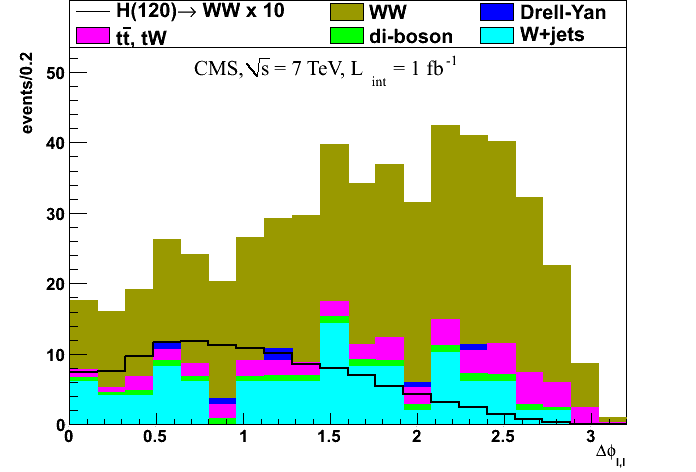
\includegraphics[width=.32\textwidth]{figures/dPhi_hm120_jets0.png}}
\subfigure[]{
\centering
\label{subfig:dPhi_hm160_jets0}
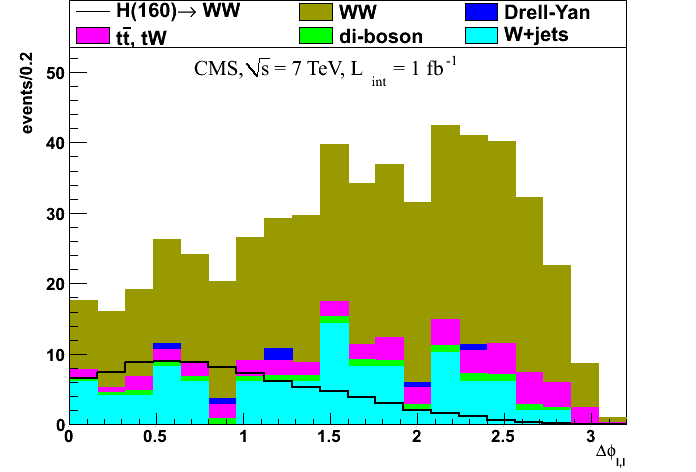
\includegraphics[width=.32\textwidth]{figures/dPhi_hm160_jets0.png}}
\subfigure[]{
\centering
\label{subfig:dPhi_hm250_jets0}
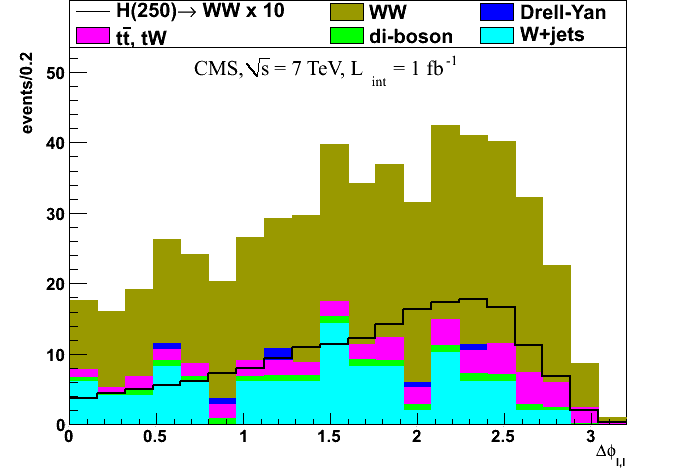
\includegraphics[width=.32\textwidth]{figures/dPhi_hm250_jets0.png}}\\
\caption{Lepton $\Delta\phi$ distribution after \WW\ selection for $m_H$=120 $\GeVcc$ \subref{subfig:dPhi_hm120_jets0}, 
$m_H$=160 $\GeVcc$ \subref{subfig:dPhi_hm160_jets0} and $m_H$=250 $\GeVcc$ \subref{subfig:dPhi_hm250_jets0} in the 0-jet bin.}
\label{fig:dPhi_jets0}
\end{figure}

\begin{figure}[!hbtp]
\centering
\subfigure[]{
\centering
\label{subfig:dilepmass_hm120_jets0}
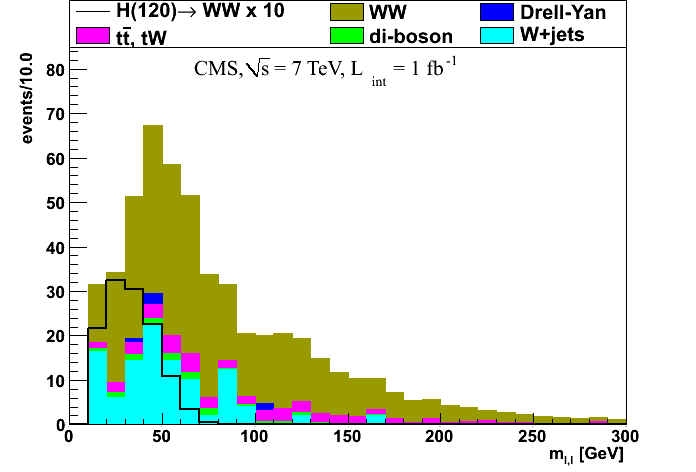
\includegraphics[width=.32\textwidth]{figures/dilepmass_hm120_jets0.png}}
\subfigure[]{
\centering
\label{subfig:dilepmass_hm160_jets0}
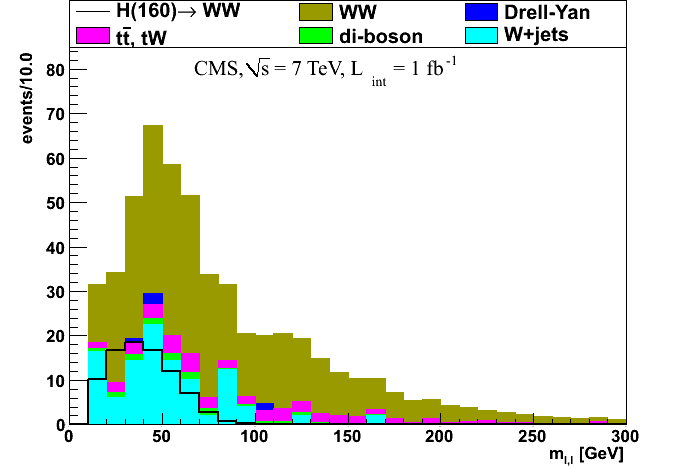
\includegraphics[width=.32\textwidth]{figures/dilepmass_hm160_jets0.png}}
\subfigure[]{
\centering
\label{subfig:dilepmass_hm250_jets0}
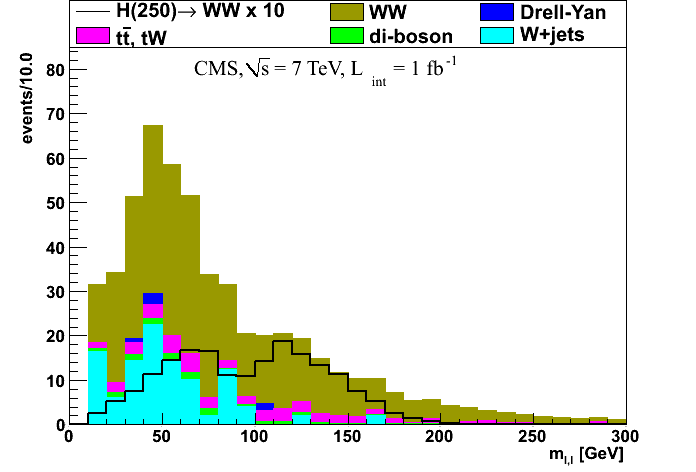
\includegraphics[width=.32\textwidth]{figures/dilepmass_hm250_jets0.png}}\\
\caption{Di-lepton mass distribution after \WW\ selection for $m_H$=120 $\GeVcc$ \subref{subfig:dilepmass_hm120_jets0}, 
$m_H$=160 $\GeVcc$ \subref{subfig:dilepmass_hm160_jets0} and $m_H$=250 $\GeVcc$ \subref{subfig:dilepmass_hm250_jets0} in the 0-jet bin.}
\label{fig:dilepmass_jets0}
\end{figure}

\begin{figure}[!hbtp]
\centering
\subfigure[]{
\centering
\label{subfig:dileppt_hm120_jets0}
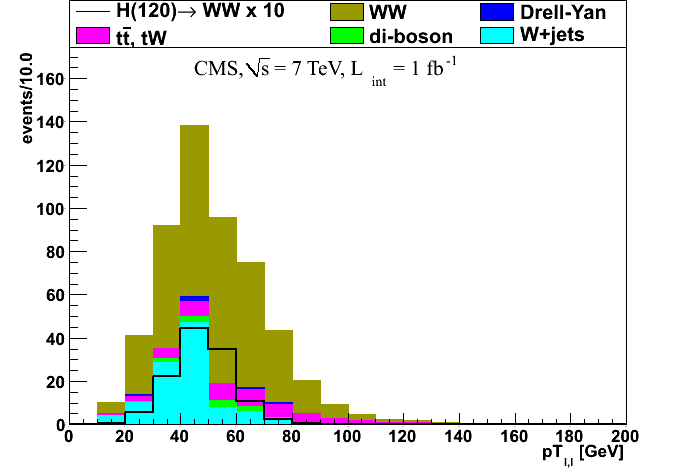
\includegraphics[width=.32\textwidth]{figures/dileppt_hm120_jets0.png}}
\subfigure[]{
\centering
\label{subfig:dileppt_hm160_jets0}
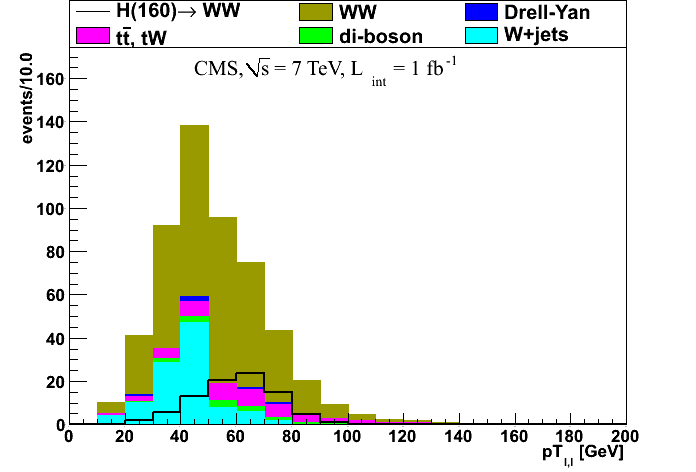
\includegraphics[width=.32\textwidth]{figures/dileppt_hm160_jets0.png}}
\subfigure[]{
\centering
\label{subfig:dileppt_hm250_jets0}
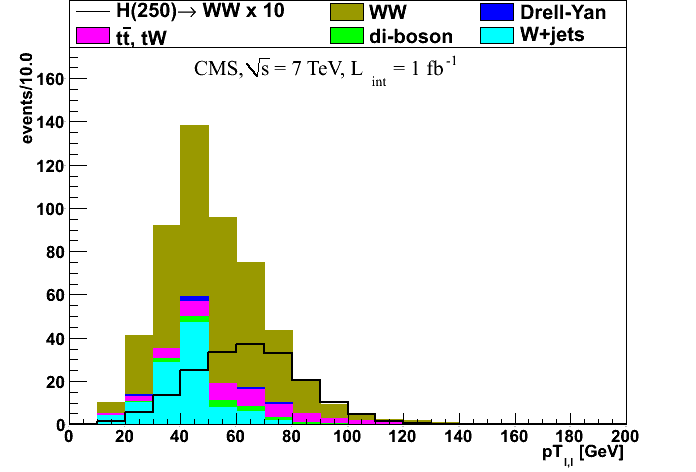
\includegraphics[width=.32\textwidth]{figures/dileppt_hm250_jets0.png}}\\
\caption{Di-lepton $p_T$ distribution after \WW\ selection for $m_H$=120 $\GeVcc$ \subref{subfig:dileppt_hm120_jets0}, 
$m_H$=160 $\GeVcc$ \subref{subfig:dileppt_hm160_jets0} and $m_H$=250 $\GeVcc$ \subref{subfig:dileppt_hm250_jets0} in the 0-jet bin.}
\label{fig:dileppt_jets0}
\end{figure}

\begin{figure}[!hbtp]
\centering
\subfigure[]{
\centering
\label{subfig:mt_hm120_jets0}
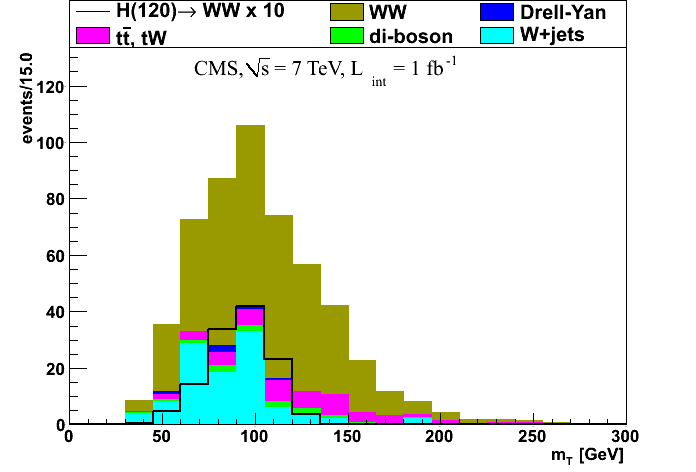
\includegraphics[width=.32\textwidth]{figures/mt_hm120_jets0.png}}
\subfigure[]{
\centering
\label{subfig:mt_hm160_jets0}
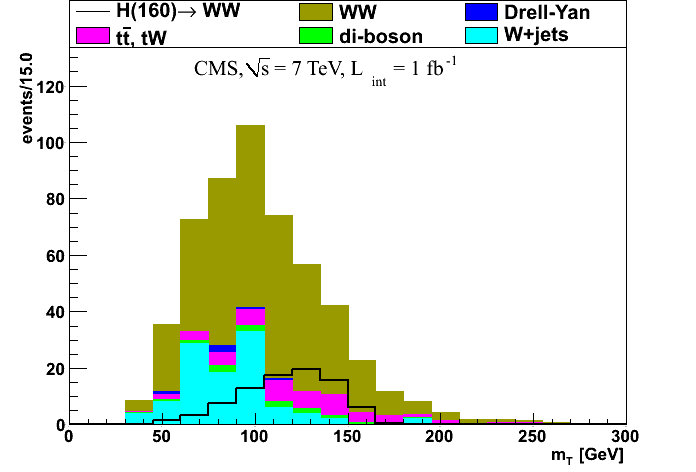
\includegraphics[width=.32\textwidth]{figures/mt_hm160_jets0.png}}
\subfigure[]{
\centering
\label{subfig:mt_hm250_jets0}
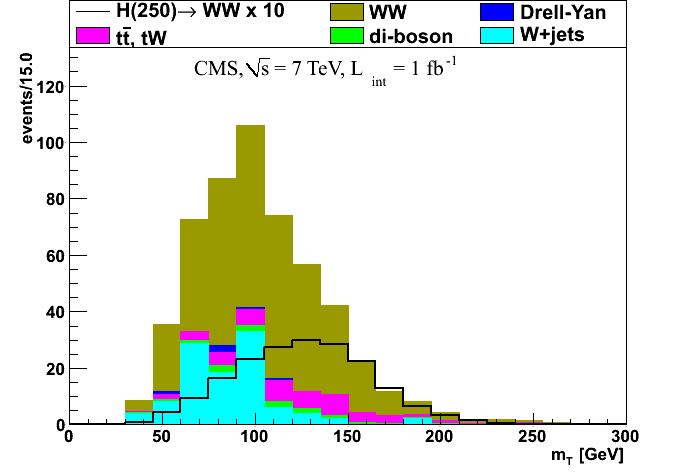
\includegraphics[width=.32\textwidth]{figures/mt_hm250_jets0.png}}\\
\caption{$m_T$ distribution after \WW\ selection for $m_H$=120 $\GeVcc$ \subref{subfig:mt_hm120_jets0}, 
$m_H$=160 $\GeVcc$ \subref{subfig:mt_hm160_jets0} and $m_H$=250 $\GeVcc$ \subref{subfig:mt_hm250_jets0} in the 0-jet bin.}
\label{fig:mt_jets0}
\end{figure}

\begin{figure}[!hbtp]
\centering
\subfigure[]{
\centering
\label{subfig:pmet_hm120_jets0}
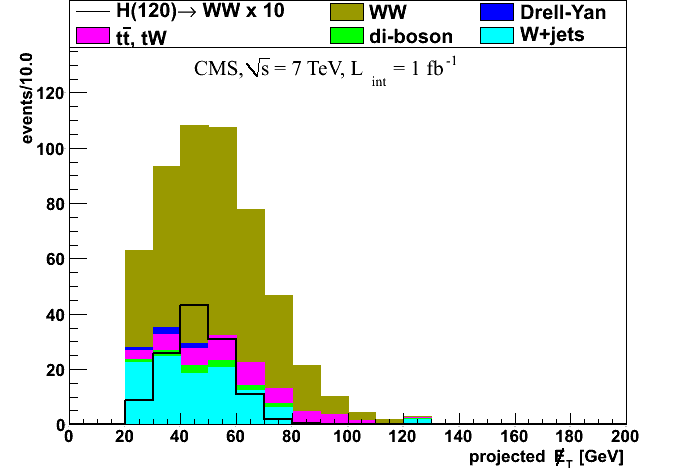
\includegraphics[width=.32\textwidth]{figures/pmet_hm120_jets0.png}}
\subfigure[]{
\centering
\label{subfig:pmet_hm160_jets0}
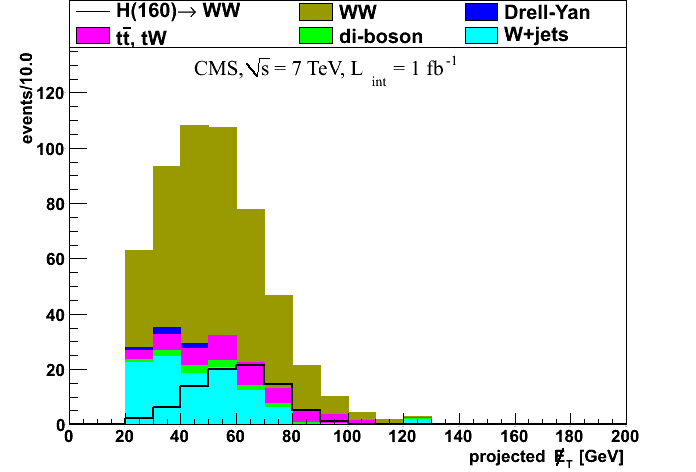
\includegraphics[width=.32\textwidth]{figures/pmet_hm160_jets0.png}}
\subfigure[]{
\centering
\label{subfig:pmet_hm250_jets0}
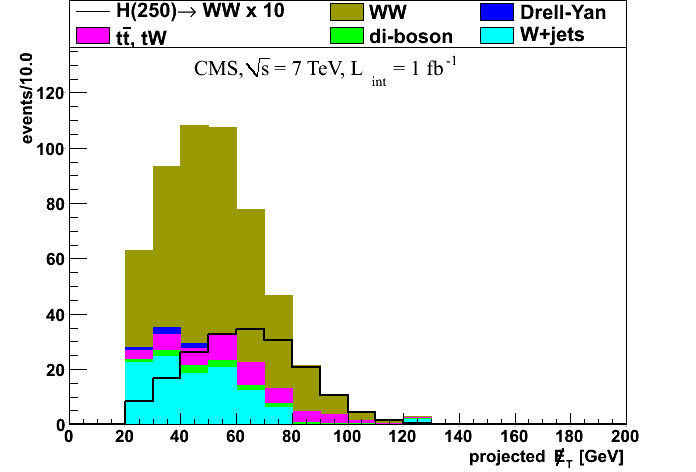
\includegraphics[width=.32\textwidth]{figures/pmet_hm250_jets0.png}}\\
\caption{Projected $\met$ distribution after \WW\ selection for $m_H$=120 $\GeVcc$ \subref{subfig:pmet_hm120_jets0}, 
$m_H$=160 $\GeVcc$ \subref{subfig:pmet_hm160_jets0} and $m_H$=250 $\GeVcc$ \subref{subfig:pmet_hm250_jets0} in the 0-jet bin.}
\label{fig:pmet_jets0}
\end{figure}








\begin{figure}[!hbtp]
\centering
\subfigure[]{
\centering
\label{subfig:dPhi_hm120_jets1}
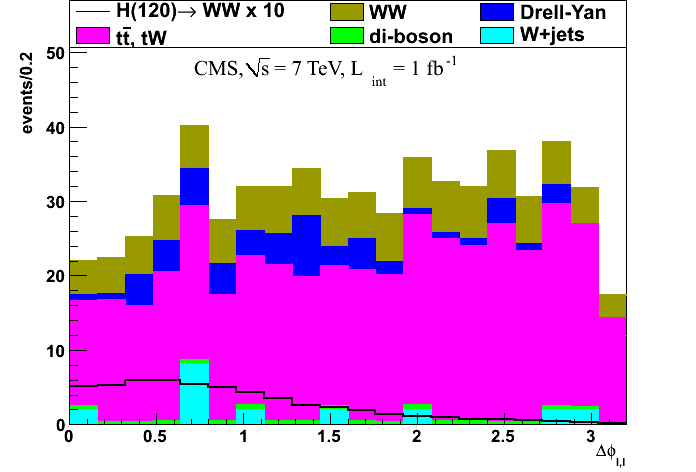
\includegraphics[width=.32\textwidth]{figures/dPhi_hm120_jets1.png}}
\subfigure[]{
\centering
\label{subfig:dPhi_hm160_jets1}
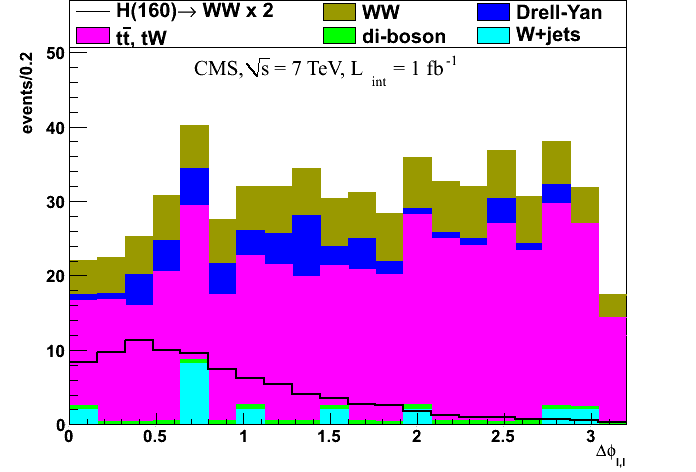
\includegraphics[width=.32\textwidth]{figures/dPhi_hm160_jets1.png}}
\subfigure[]{
\centering
\label{subfig:dPhi_hm250_jets1}
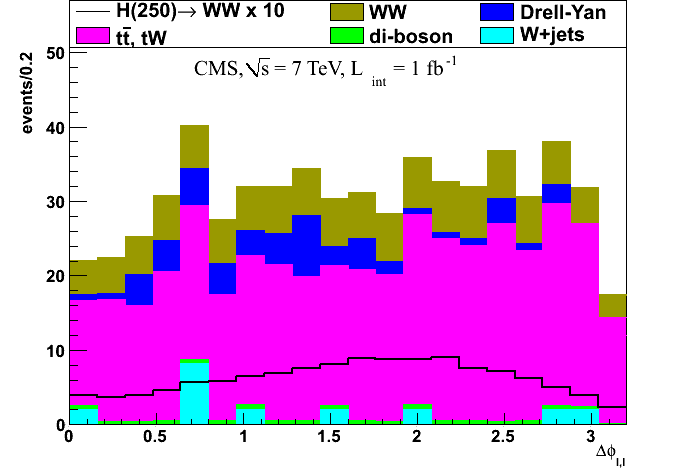
\includegraphics[width=.32\textwidth]{figures/dPhi_hm250_jets1.png}}\\
\caption{Lepton $\Delta\phi$ distribution after \WW\ selection for $m_H$=120 $\GeVcc$ \subref{subfig:dPhi_hm120_jets1}, 
$m_H$=160 $\GeVcc$ \subref{subfig:dPhi_hm160_jets1} and $m_H$=250 $\GeVcc$ \subref{subfig:dPhi_hm250_jets1} in the 1-jet bin.}
\label{fig:dPhi_jets1}
\end{figure}

\begin{figure}[!hbtp]
\centering
\subfigure[]{
\centering
\label{subfig:dilepmass_hm120_jets1}
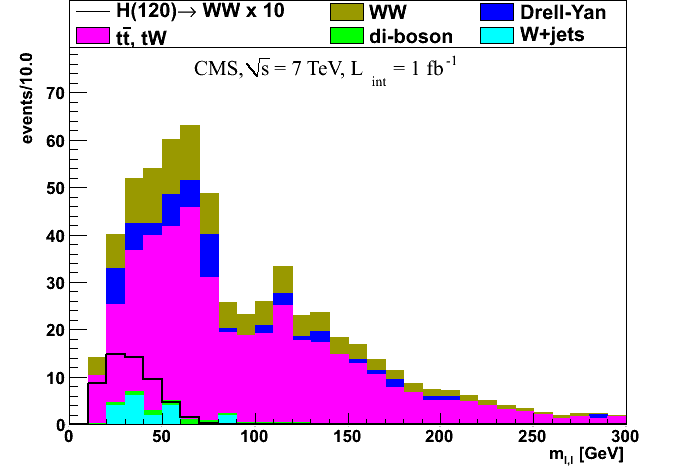
\includegraphics[width=.32\textwidth]{figures/dilepmass_hm120_jets1.png}}
\subfigure[]{
\centering
\label{subfig:dilepmass_hm160_jets1}
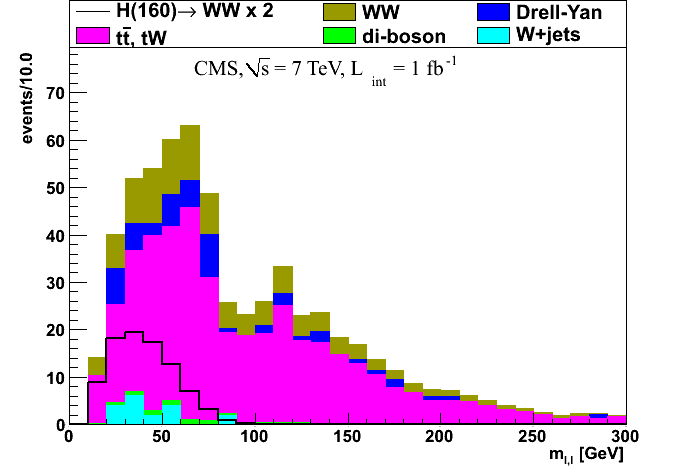
\includegraphics[width=.32\textwidth]{figures/dilepmass_hm160_jets1.png}}
\subfigure[]{
\centering
\label{subfig:dilepmass_hm250_jets1}
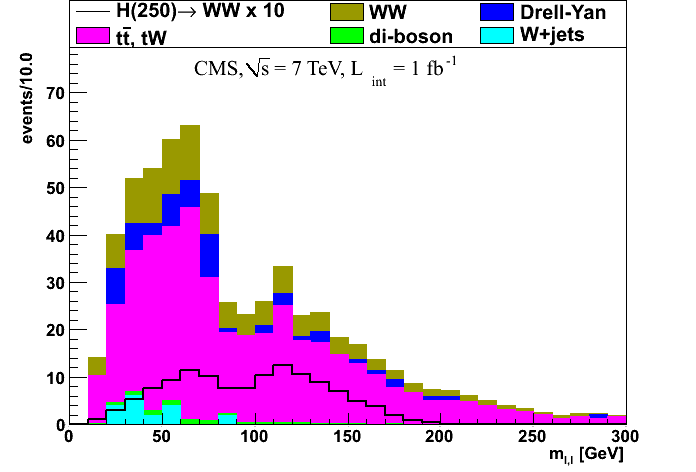
\includegraphics[width=.32\textwidth]{figures/dilepmass_hm250_jets1.png}}\\
\caption{Di-lepton mass distribution after \WW\ selection for $m_H$=120 $\GeVcc$ \subref{subfig:dilepmass_hm120_jets1}, 
$m_H$=160 $\GeVcc$ \subref{subfig:dilepmass_hm160_jets1} and $m_H$=250 $\GeVcc$ \subref{subfig:dilepmass_hm250_jets1} in the 1-jet bin.}
\label{fig:dilepmass_jets1}
\end{figure}

\begin{figure}[!hbtp]
\centering
\subfigure[]{
\centering
\label{subfig:dileppt_hm120_jets1}
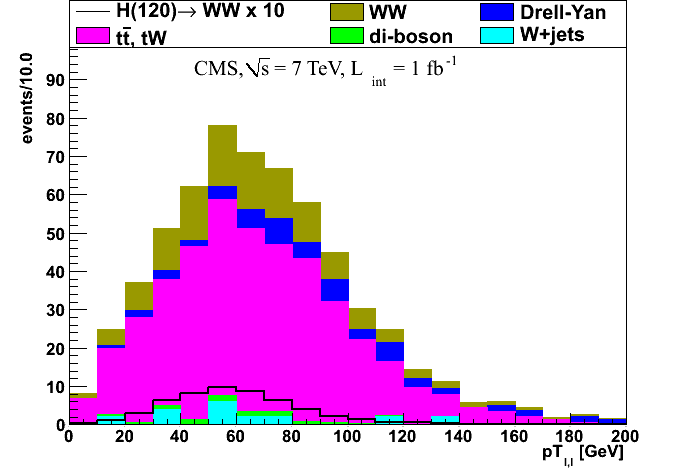
\includegraphics[width=.32\textwidth]{figures/dileppt_hm120_jets1.png}}
\subfigure[]{
\centering
\label{subfig:dileppt_hm160_jets1}
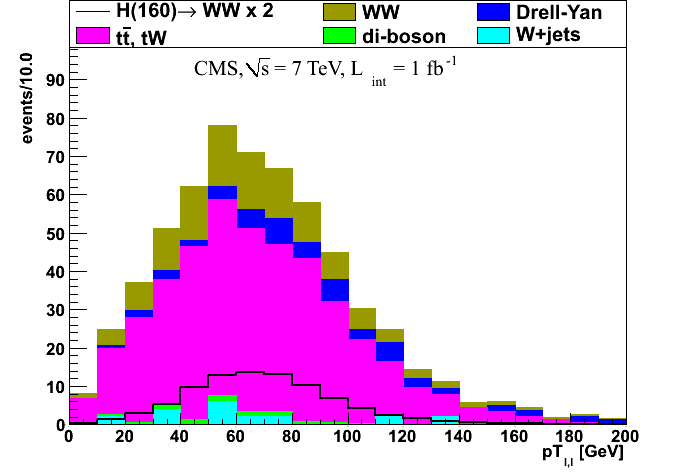
\includegraphics[width=.32\textwidth]{figures/dileppt_hm160_jets1.png}}
\subfigure[]{
\centering
\label{subfig:dileppt_hm250_jets1}
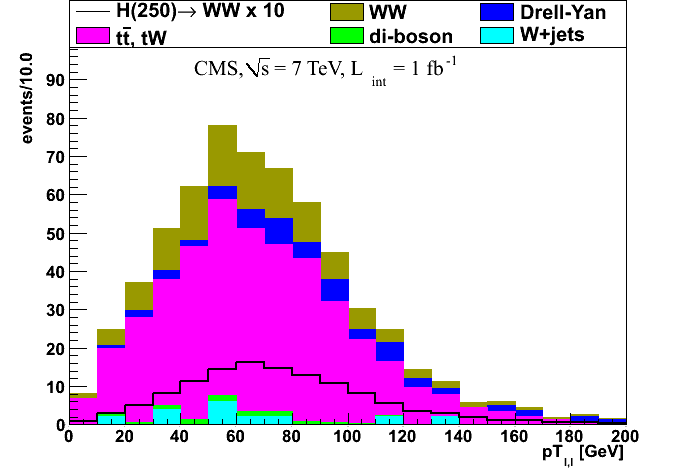
\includegraphics[width=.32\textwidth]{figures/dileppt_hm250_jets1.png}}\\
\caption{Di-lepton $p_T$ distribution after \WW\ selection for $m_H$=120 $\GeVcc$ \subref{subfig:dileppt_hm120_jets1}, 
$m_H$=160 $\GeVcc$ \subref{subfig:dileppt_hm160_jets1} and $m_H$=250 $\GeVcc$ \subref{subfig:dileppt_hm250_jets1} in the 1-jet bin.}
\label{fig:dileppt_jets1}
\end{figure}

\begin{figure}[!hbtp]
\centering
\subfigure[]{
\centering
\label{subfig:mt_hm120_jets1}
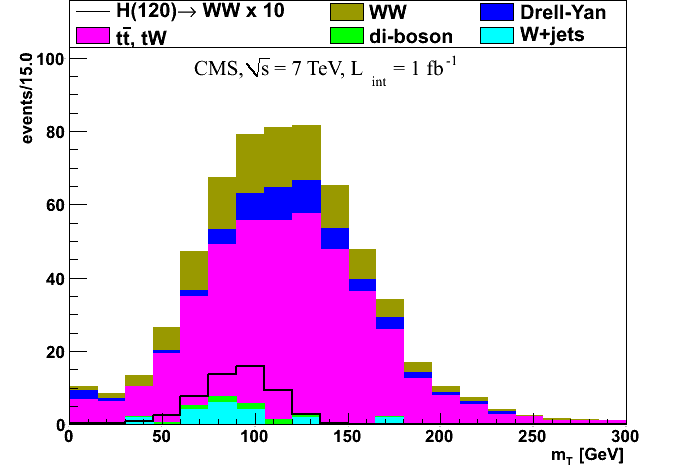
\includegraphics[width=.32\textwidth]{figures/mt_hm120_jets1.png}}
\subfigure[]{
\centering
\label{subfig:mt_hm160_jets1}
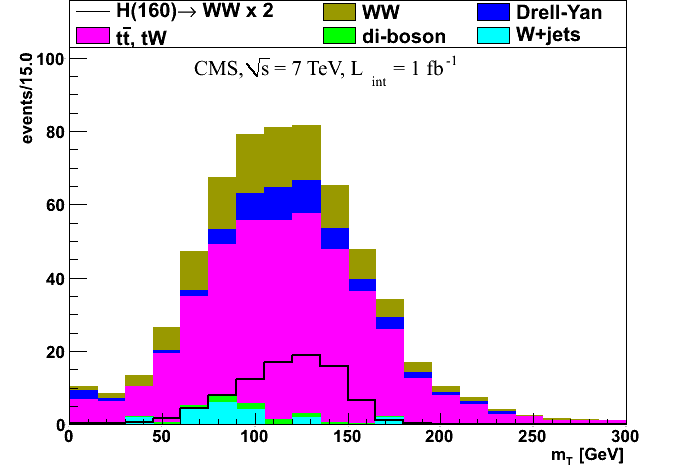
\includegraphics[width=.32\textwidth]{figures/mt_hm160_jets1.png}}
\subfigure[]{
\centering
\label{subfig:mt_hm250_jets1}
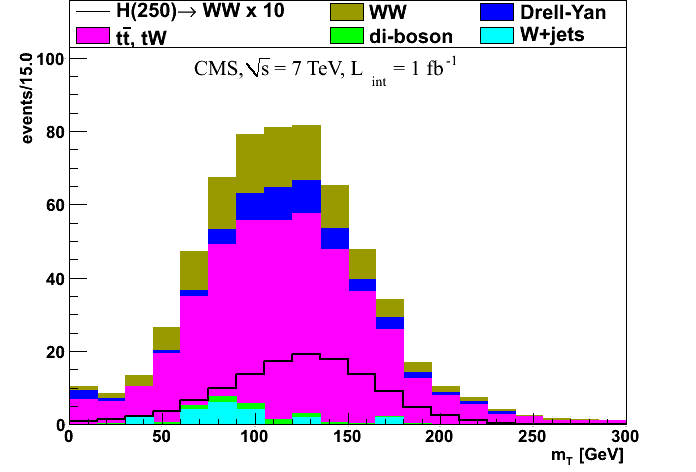
\includegraphics[width=.32\textwidth]{figures/mt_hm250_jets1.png}}\\
\caption{$m_T$ distribution after \WW\ selection for $m_H$=120 $\GeVcc$ \subref{subfig:mt_hm120_jets1}, 
$m_H$=160 $\GeVcc$ \subref{subfig:mt_hm160_jets1} and $m_H$=250 $\GeVcc$ \subref{subfig:mt_hm250_jets1} in the 1-jet bin.}
\label{fig:mt_jets1}
\end{figure}

\begin{figure}[!hbtp]
\centering
\subfigure[]{
\centering
\label{subfig:pmet_hm120_jets1}
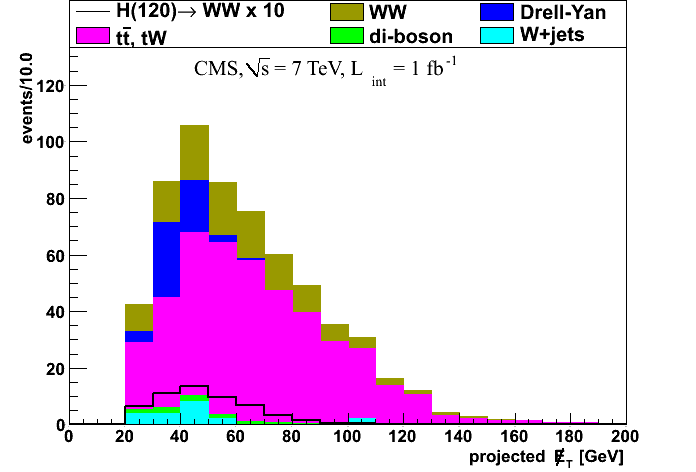
\includegraphics[width=.32\textwidth]{figures/pmet_hm120_jets1.png}}
\subfigure[]{
\centering
\label{subfig:pmet_hm160_jets1}
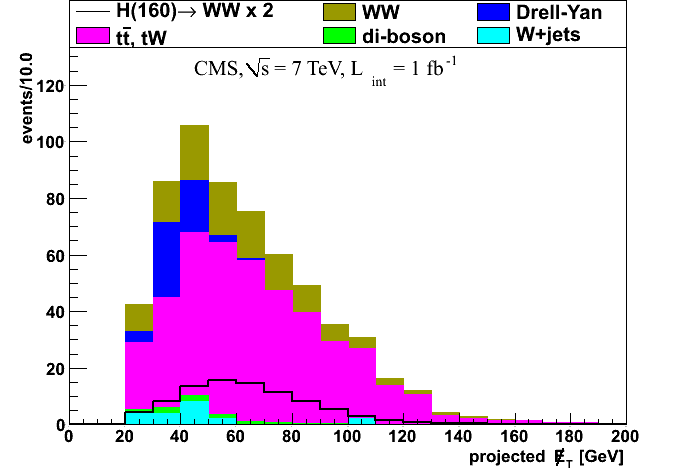
\includegraphics[width=.32\textwidth]{figures/pmet_hm160_jets1.png}}
\subfigure[]{
\centering
\label{subfig:pmet_hm250_jets1}
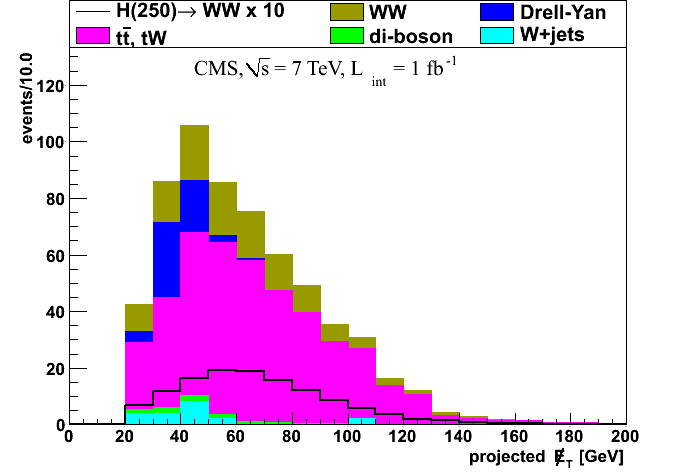
\includegraphics[width=.32\textwidth]{figures/pmet_hm250_jets1.png}}\\
\caption{Projected $\met$ distribution after \WW\ selection for $m_H$=120 $\GeVcc$ \subref{subfig:pmet_hm120_jets1}, 
$m_H$=160 $\GeVcc$ \subref{subfig:pmet_hm160_jets1} and $m_H$=250 $\GeVcc$ \subref{subfig:pmet_hm250_jets1} in the 1-jet bin.}
\label{fig:pmet_jets1}
\end{figure}
